\section{Execution}
\label{sc:execution}




%DESENHO DA ARQUITETURA DO Sistema.

Figure \ref{fig:arch} shows the execution of the benchmark and measurements of energy consumption of \gls{dbms}, where it displays the architecture of our energy benchmarking system and the flow of actions.



%Imagem
\begin{figure}[H]
  \centering
  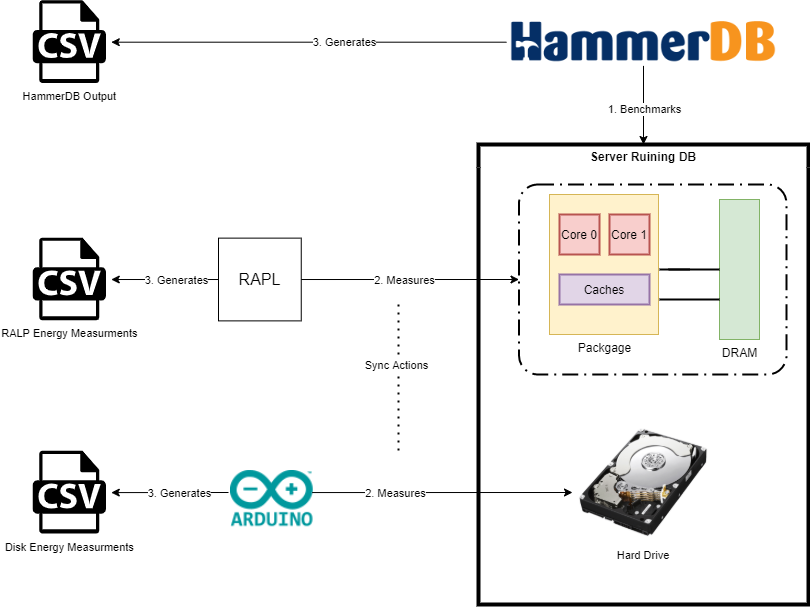
\includegraphics[width=\linewidth]{Chapters/images/arquitetura.png}
      \caption{Benchmark Architecture and flow of events}
  \label{fig:arch}
\end{figure}

% Explicar 1º Passo% cada script foi executado 10 vezes



As seen in Figure \ref{fig:arch}, the first action of our execution is the Benchmark initialization and execution of HammerDB. To obtain proper and reliable energy readings, we needed to diminish the effects of cold starts, warm-ups, cache effects, and other effects that may influence energy consumption. So, each scenario is executed ten times with a sleep time of 2 minutes between each execution.

%In order to have proper energy readings, we need to reduce the effects of cold starts, warm-ups, cache effects, and other effects that may influence energy consumption. Thus, each script is executed 10 times with a sleep time of 2 minutes between each execution.


%Sample do Arduino e RAPL

Immediately after the start of the Benchmark execution, The measurements of the energy consumption start. The framework tools used were the ones mentioned in Section \ref{energyframe}.  In the case of the \gls{rapl}, the sample used was 100 measurements per second, and for the Arduino was ten measures per second.

%Explicar o RAPLSERVER que foi usado para sync as mediçoes entre o Arduino e o RAPL.

These two measurement tools are in sync throughout the entire execution. We accomplished this by using a C program that starts two independent sync threads: one that accesses the \gls{rapl} to measure the \gls{cpu} is power consumption, and the other accesses the Arduino to measure the disk's power consumption. They are active during the execution of HammerDB and accumulate energy readings in static arrays to limit their computing overhead.


%3fase

The third and final phase of our execution begins after the HammerDB execution is completed. This step saves each measurement mad in its respective CSV file for further analysis.



%Para reduzir os vestigios e faciltar montar diferentes dbms foi usado DOCKER


Also, for each database, we decide to use dockers containers because it is a solution that simplifies the setup by providing a pre-built image that is portable, simple to maintain, and providing a facility to automate the applications when they are deployed into containers~\cite{rad2017introduction,10.1145/2723872.2723882}. Although several studies recognize that dockers provide an overhead in running these containers~\cite{chung2016using,varghese2016container,impactDocker,felter2015updated}, dockerized benchmarks can be acceptable when comparing different database systems if the idle consumption values are disregarded~\cite{grambow2019safe}.


%System Configuration
\paragraph{System Configuration}

We ran this study on a server with the following specifications presented in Table  \ref{Tab:physicalserver}, this consists of an Intel(R) Core i5-4460 3.28 GHz \gls{cpu}, 16 GB of \gls{ram}, 250 GB \gls{hdd}, and operating system Ubuntu 16.10 . A detailed overview of the \gls{cpu} is in Table \ref{tab:cpuspec} and for Second Storage is in Table \ref{tab:diskspec}.

\begin{table}[H]
\centering
\begin{tabular}{|c|c|}
\hline
Hardware               & Model \\ \hline
CPU                    & Intel(R) Core i5-4460 3.28 GHz   \\ \hline
Operation System       & Ubuntu 16.10   \\ \hline
Ram Size               & 16G   \\ \hline
Secondary Storage      & Hitachi Travelstar 250 GB   \\ \hline
\end{tabular}
\caption{Physical server specifications}
\label{Tab:physicalserver}

\end{table}

    \begin{table}[!ht]
    \centering
\begin{minipage}[t]{0.48\linewidth}\centering
\begin{tabular}{|c|c|}
\hline
\multicolumn{2}{|c|}{CPU}      \\ \hline
Brand               & Intel    \\ \hline
Model               & i5-4460  \\ \hline
Microarchitecture   & Haswell  \\ \hline
Number of cores     & 4        \\ \hline
Clock Speed         & 3.20 GHz \\ \hline
Max Turbo Frequency & 3.40 GHz \\ \hline
Cache               & 6 MB     \\ \hline
Interface           & Sata 3   \\ \hline
Buffer Size         & 8MB      \\ \hline
\end{tabular}
\caption{Specifications of CPU used}\label{tab:cpuspec}
\end{minipage}\hfill%
\begin{minipage}[t]{0.48\linewidth}\centering
\begin{tabular}{|c|c|}
\hline
\multicolumn{2}{|c|}{Second Storage} \\ \hline
Brand          & Hitachi GST         \\ \hline
Model          & HTE543225A7A384     \\ \hline
Series         & Travelstar Z5K320   \\ \hline
Type           & HDD                 \\ \hline
Capacity       & 250 GB              \\ \hline
RPM            & 5400                \\ \hline
Interface      & Sata 3              \\ \hline
Buffer Size    & 8MB                 \\ \hline
\end{tabular}
\caption{Specifications of Disk used}\label{tab:diskspec}
\end{minipage}
\end{table}

%

\begin{table}[H]
\centering
\begin{tabular}{|c|c|}
\hline
\multicolumn{2}{|c|}{CPU}      \\ \hline
Brand               & Intel    \\ \hline
Model               & i5-4460  \\ \hline
Microarchitecture   & Haswell  \\ \hline
Number of cores     & 4        \\ \hline
Clock Speed         & 3.20 GHz \\ \hline
Max Turbo Frequency & 3.40 GHz \\ \hline
Cache               & 6 MB     \\ \hline
Interface           & Sata 3   \\ \hline
Buffer Size         & 8MB      \\ \hline
\end{tabular}
\caption{Specifications of CPU used}\label{tab:cpuspec}

\end{table}


%
\begin{table}[H]
%https://www.newegg.com/hitachi-gst-travelstar-z5k320-250gb-hte543225a7a384/p/N82E16822145458
\centering
\begin{tabular}{|c|c|}
\hline
\multicolumn{2}{|c|}{Second Storage} \\ \hline
Brand          & Hitachi GST         \\ \hline
Model          & HTE543225A7A384     \\ \hline
Series         & Travelstar Z5K320   \\ \hline
Type           & HDD                 \\ \hline
Capacity       & 250 GB              \\ \hline
RPM            & 5400                \\ \hline
Interface      & Sata 3              \\ \hline
Buffer Size    & 8MB                 \\ \hline
\end{tabular}
\caption{Specifications of Disk used}\label{tab:diskspec}

\end{table}

This system has no additional software installed or running other than required to run this research. Additionally, we had the caution to use the most recent and compatible version of all external software used here at the time of the measurements. So listed in Table \ref{Tab:softwareconfig} are all the versions used.

\begin{table}[H]
\centering
\begin{tabular}{|c|c|}
\hline
Software & Version \\ \hline
Redis    &  5.0.5  \\ \hline
Postgres &  11.5   \\ \hline
MySQL    &  8.0    \\ \hline
MariaDB  &  10.0      \\ \hline
HammerDB  &  3.2   \\ \hline
Docker & 19.03.11 \\ \hline
\end{tabular}
\caption{Software Configuration on physical server}
\label{Tab:softwareconfig}

\end{table}





All software artifacts shown in Figure~\ref{fig:arch} and mention in this chapter, are  available as a public repository at \url{https://github.com/greensoftwarelab/GreenSGDBS}.
